\chapter{Έλεγχος Ποιότητας}

\section{Εισαγωγή}
Καθώς το σύστημα μας μεγαλώνει συνεχώς και οι έννοιες γίνονται όλο και πιο σύνθετες οφείλουμε να ελέγχουμε αν όλες οι λειτουργίες δουλεύουν όπως αναμένουμε. Για να γίνει αυτό δημιουργήθηκαν test στα επιμέρους συστήματα για τον έλεγχο των διάφορων κομματιών του κώδικά μας. Παρακάτω θα παρουσιάσουμε τα εργαλεία που χρησιμοποιήθηκαν όπως επίσης και μερικά παραδείγματα για να γίνει ξεκάθαρος ο τρόπος με τον οποίο ελέγχθηκε η λειτουργικότητα του συστήματος.

\section{Unit Testing}
Μία από τις πιο βασικές έννοιες στον έλεγχο ποιότητας είναι το Unit Testing. Σκοπός των unit tests είναι ο έλεγχος λειτουργίας ενός συγκεκριμένου κομματιού κώδικα και τις λογικής την οποία αυτό εκφράζει. Έτσι δημιουργείτε μια απομόνωση των διάφορων λειτουργιών και ο έλεγχος τους γίνεται πιο εύκολος. Παρακάτω θα αναφερθούμε στα εργαλεία που χρησιμοποιήθηκαν για τη δημιουργία unit tests στις εφαρμογές μας καθώς και στον εξυπηρετητή.

\subsection{Εφαρμογές}
Όπως έχουμε προαναφέρει, η εφαρμογή κινητών συσκευών καθώς και η διαδικτυακή εφαρμογή αναπτύχθηκαν με τη χρήση του Angular framework. Το Angular framework έχει γραφτεί έχοντας κατά νου τις βασικές αρχές του ελέγχου ποιότητας. Έτσι υπάρχουν εργαλεία τα οποία βοηθούν στη δημιουργία test, όπως το Jasmine framework. 

\subsubsection{Jasmine Framework}
Το Jasmine framework έχει ως γνώμονα τη συμπεριφορά που αναμένεται κατά της διάρκεια του ελέγχου του κώδικα (behavior-driven) έτσι διευκολύνει τη δημιουργία των test. Για να γίνει αυτό αντιληπτό παρακάτω θα παρουσιάσουμε ένα απλό test στο οποίο ελέγχουμε αν ο αλγόριθμος της κρυπτογράφησης των δεδομένων του χρήστη συμπεριφέρεται όπως αναμένουμε.

\begin{lstlisting}[language=Java, caption=Jasmine test, label={lst:jasmine-test}]
describe('LoginController', function() {
  beforeEach(module('tracegerm'));
  var $controller;

  beforeEach(inject(function(_$controller_){
    $controller = _$controller_;
  }));

  describe('#DoEncryption', function() {
    it('checks the encryption', function() {
      var $scope = {};
      var controller = $controller('LoginController', { $scope: $scope });
      $scope.registerInfo.password = 'longerthaneightchars';

      var value = "value";
      var encryptedvalue = $scope.encryptValue(value);
      var text = CryptoJS.AES.decrypt(encryptedvalue.toString(), 
      $scope.registerInfo.password).toString(CryptoJS.enc.Utf8);
      
      expect(value).toEqual(text);
    });
  })
});
\end{lstlisting}

\section{Εξυπηρετητής}
Εφόσον ο εξυπηρετητής έχει γραφθεί με τη γλώσσα Java δημιουργήσαμε test για τον έλεγχο ποιότητας με το JUnit framework.

\subsubsection{Junit Framework}
Το JUnit framework είναι ίσως το πιο διαδεδομένο εργαλείο ελέγχου ποιότητας στη γλώσσα Java. Όπως κάθε εργαλείο για unit testing έχει σαν στόχο τον έλεγχο ενός βασικού μέρους του κώδικα και να συγκρίνει το αποτέλεσμα με τα δεδομένα με τα οποία αναμένουμε. Παρακάτω θα εμφανίσουμε ένα απλό παράδειγμα test στο οποίο ελέγχουμε αν ανακτούμε μονάχα τους συναγερμούς ενός χρήστη οι οποίοι δεν έχουν γίνει ακόμα αποδεκτοί.

\begin{lstlisting}[language=Java, caption=JUnit test, label={lst:junit-test}]
@ActiveProfiles("test")
@RunWith(SpringJUnit4ClassRunner.class)
@SpringApplicationConfiguration(classes = Application.class)
public class AlertTests {


    @Autowired
    private AlertRepository alertRepository;

    @Autowired
    private UserRepository userRepository;

    @Before
    public void setup() {
        User user = new User();
        user.setUsername("user");
        user.setPassword("user");
        userRepository.save(user);
        Alert alert = new Alert();
        alert.setAccepted(false);
        alert.setUser(user);
        Date date = new Date();
        alert.setTimestamp(new Timestamp(date.getTime()));
        alertRepository.save(alert);

        Alert alert2 = new Alert();
        alert2.setAccepted(true);
        alert2.setUser(user);
        alert2.setTimestamp(new Timestamp(date.getTime()));
        alertRepository.save(alert2);
    }

    @Test
    public void testAlertsNotAccepted() {
        Assert.assertEquals(1, alertRepository.findAlertsByAccepted(false).size());
    }

}
\end{lstlisting}

\subsection{Αποτελέσματα ελέγχου ποιότητας}
Μετά την ολοκλήρωση εκτέλεσης των test τα εργαλεία τα οποία έχουν προαναφερθεί, δημιουργούν μία σειρά από αναφορές. Οι αναφορές αυτές, παρουσιάζουν μία λεπτομερή λίστα των test των οποίων έγινε εκτέλεση καθώς και των αποτελεσμάτων τους. Υπάρχουν πολυάριθμοι τρόποι παρουσίασης των αποτελεσμάτων όπως XML, JSON, HTML κτλ. Στη περίπτωσή μας παράγουμε τα αποτελέσματα σε μορφή HTML καθώς θεωρήθηκε η πιο εύκολα αναγνώσιμη μέθοδος. 	
Συνοψίζοντας, παρακάτω στα διαγράμματα ~\ref{fig:junit-report} και ~\ref{fig:protractor-report} μπορούμε να δούμε με λεπτομέρεια τα αποτελέσματα κάποιων από τα test τα οποία δημιουργήθηκαν για την εφαρμογή μας. 

\begin{figure}[h]
  \centering
  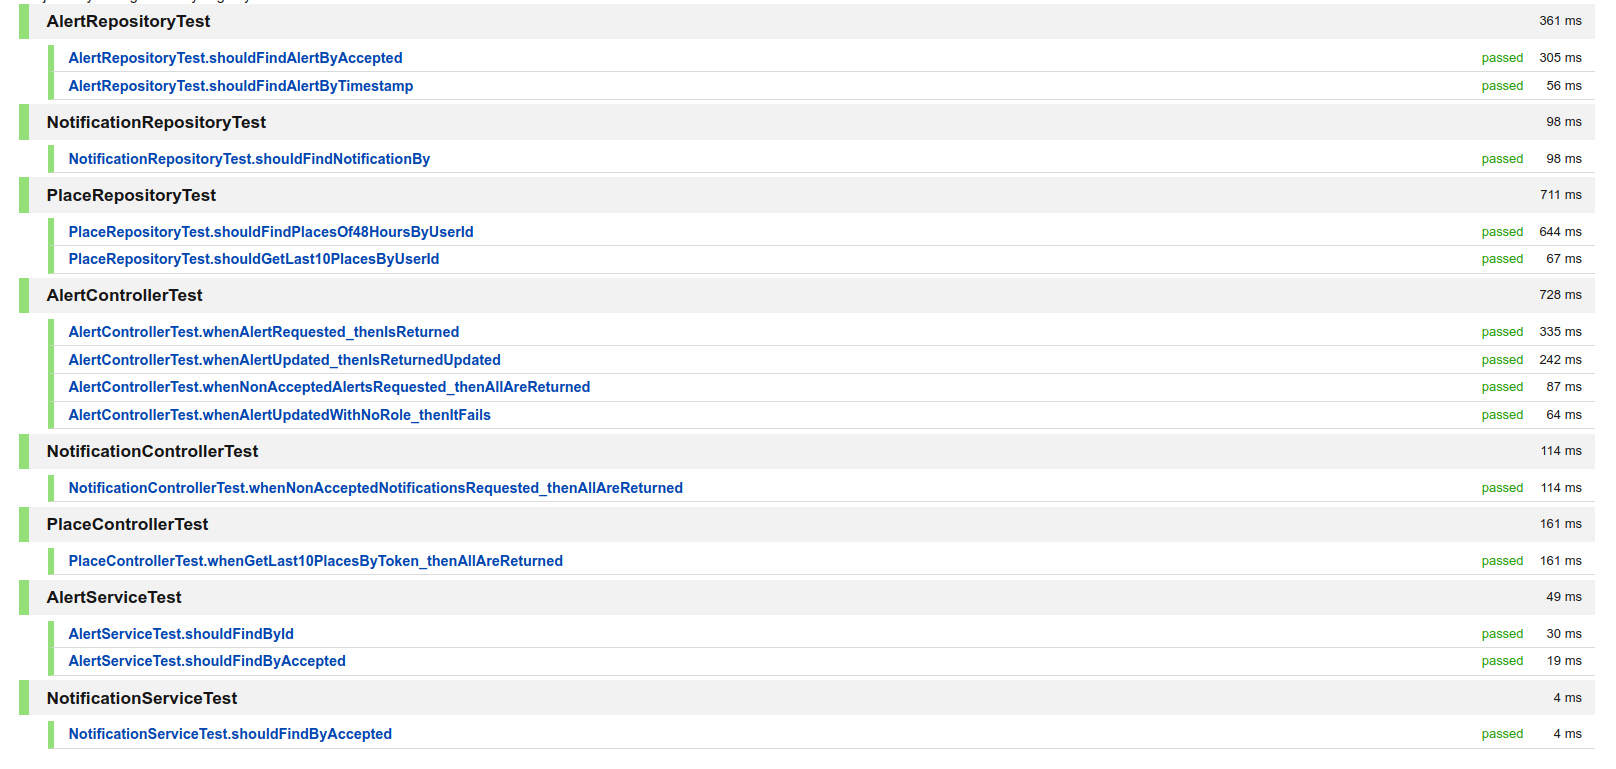
\includegraphics[width=150mm]{images/junit-report.png}
  \caption{Αναφορά Junit}
  \label{fig:junit-report}
\end{figure}

\begin{figure}[h]
  \centering
  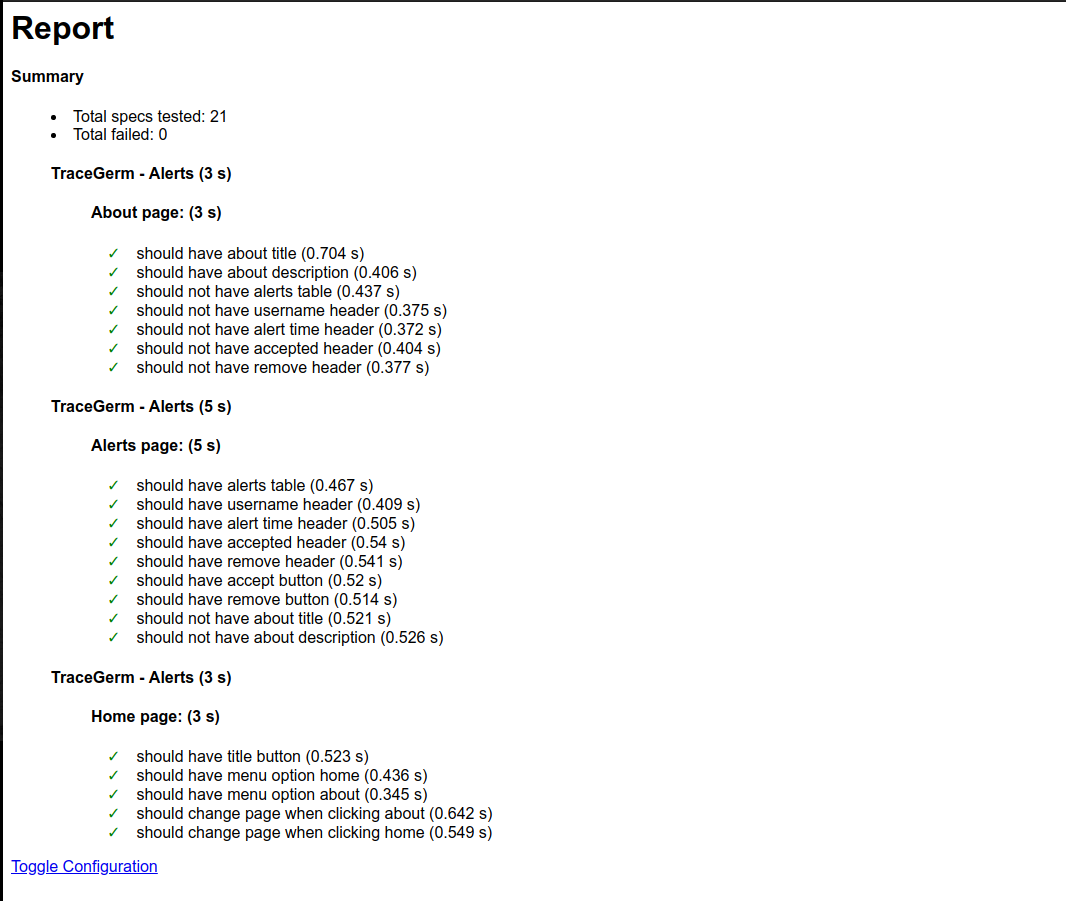
\includegraphics[width=150mm]{images/protractor-report.png}
  \caption{Αναφορά test Εφαρμογών}
  \label{fig:protractor-report}
\end{figure}